\documentclass[./main.tex]{subfiles}

\begin{document}

\chapter{BLE mesh}

\section{Introduction}
Bluetooth mesh networking provides the foundation to create a truly large-scale device network, allowing tens, hundreds or even thousands of wireless devices to communicate with each other reliably and securely.

Compared with other topologies, in a mesh network, each node may have a direct communication link with many nodes. This brings the robustness to the network against the single point of failure problem but also makes it harder to manage. Figure \ref{fig:Mesh topology} illustrates a basic example of mesh topology.

\begin{figure}[ht]
    \begin{center}
        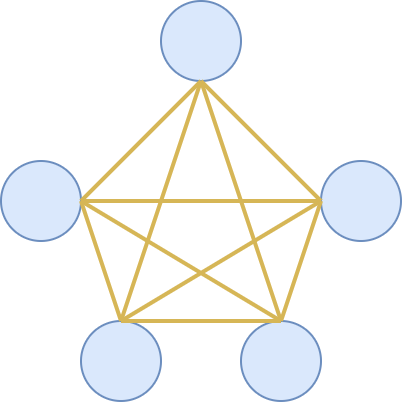
\includegraphics[scale=0.3]{mesh_topo.png}
    \end{center}
    \caption{Mesh topology}
    \label{fig:Mesh topology}
\end{figure}

A BLE mesh capable device which is not a member of any BLE mesh network is called \textbf{unprovisioned device}. After joining a  network, it is eligible to call it a \textbf{node}. The action of making an unprovisioned device become a node is called \textbf{provision}.

There may be more than one kind of node existing in a BLE mesh network. Each kind plays a different role working together to make the network run. Five types of nodes are defined in the \textbf{Mesh Networking Specifications} published by Bluetooth SIG (Bluetooth Special Interest Group).
\begin{itemize}
    \item Normal node (usually called node)
    \item Relay node
    \item Low power node
    \item Friend node
    \item Proxy node
\end{itemize}
\section{Node software architecture}
Figure \ref{fig:Node software architecture} shows the software architecture of a node. In application implementation, understanding each component is required because there are the needs of defining each of them in memory. The details of each component is discussed in the following subsection.
\begin{figure}[ht]
    \begin{center}
        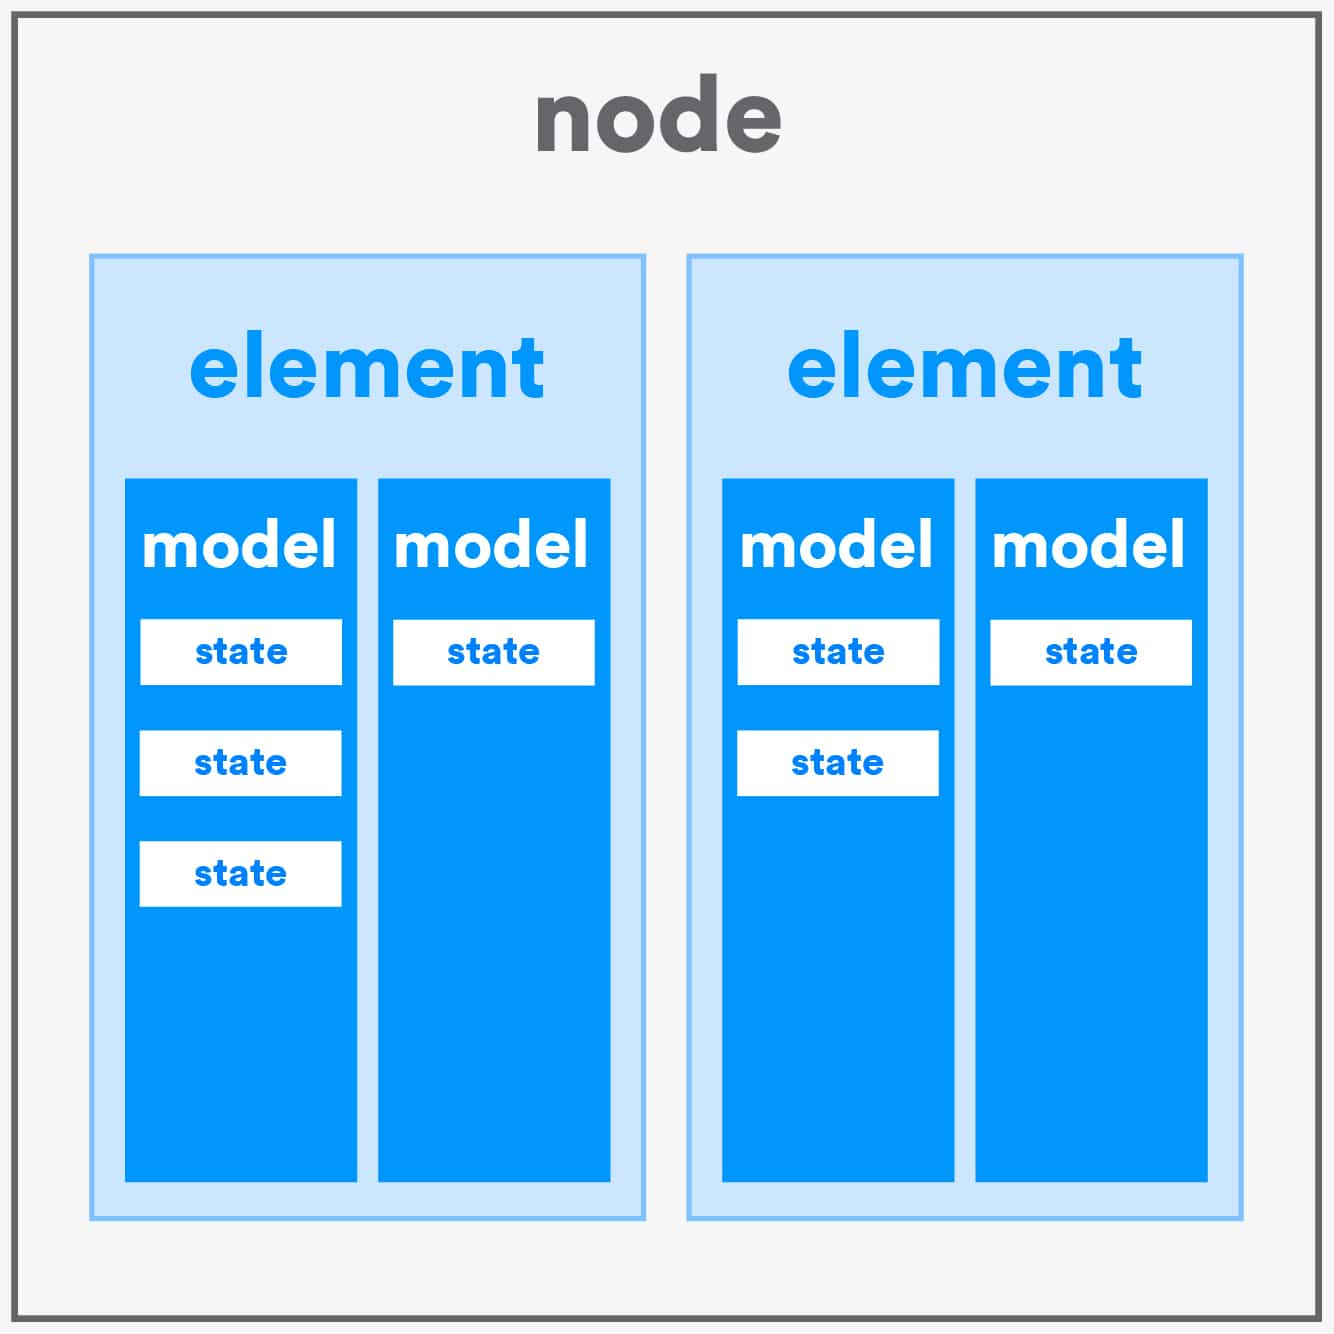
\includegraphics[scale=0.2]{node_software_architecture.jpg}
    \end{center}
    \caption{Node software architecture}
    \label{fig:Node software architecture}
\end{figure}

\subsection{Element}
In a BLE mesh network, a node is a physical device consisting of one or more elements. Compared to the node, an element is the logic component of the network. By this way, a mesh network is logically a group of elements communicating with others. Because an element is a network entity, it will be addressed uniquely in the mesh network.

Why element is defined? Let's think of a device with more than one light bulb, by introducing the element concept, each light bulb may be considered as an element of the network. This makes the network more flexible and removes application layer special muxing.

\subsection{Model}
The communication channel between elements is the model. A model can subscribe to a topic or publish data to a topic that may be subscribed by other models. The publish/subscribe pattern brings the ability to  communicate with multiple devices with a single message without knowing the exact address of such devices. Figure \ref{fig:BLE mesh publish/subscribe model} illustrates the publish/subscribe pattern. 

\begin{figure}[ht]
    \begin{center}
        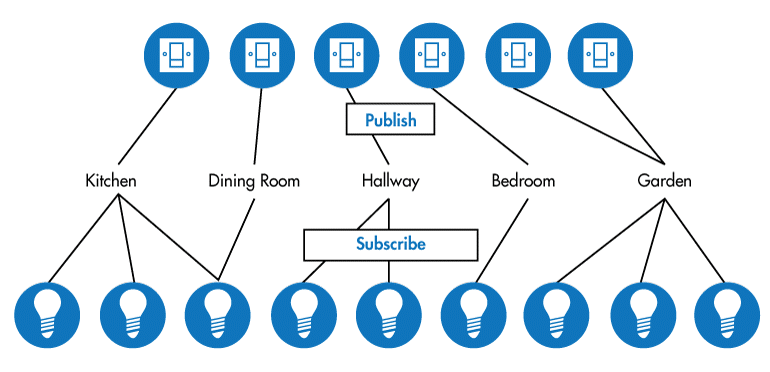
\includegraphics[scale=0.5]{ble_mesh_pub_sub.png}
    \end{center}
    \caption{BLE mesh publish/subscribe model}
    \label{fig:BLE mesh publish/subscribe model}
\end{figure}

\subsection{State}
A state is an internal variable inside the model. In the simple case, it may save a state of the element such as the on/off state of a light bulb.

\end{document}